%!TEX root =  main.tex
Sequential \ses arises in many security and healthcare diagnostic systems. In these applications we have a diverse collection of sensor-based-tests with differing costs and accuracy. %Each SBT outputs a prediction of the latent state of an instance.
In these applications (see \cref{motiv}) inexpensive tests are first conducted and based on their outcomes a decision for acquiring more (expensive) tests are made. %For instance, in security systems a number of different imaging and non-imaging tests are sequentially processed (see \cite{ML13_MultistageClassifier_TrapezSaligramaCastanon}). Costs can arise due to sensor availability and delay (see Fig.~\ref{motiv}). %A suite of SBTs ranging from inexpensive/rapid tests to more expensive/slow tests are employed. SBTs, as depicted in Fig.~\ref{motiv}, are typically organized in a hierarchical architecture resulting in sequential \ses of low-cost low-accuracy tests first followed by more expensive higher-accuracy tests. %The task is to determine which tests lead to maximizing accuracy for the available cost-budget. test for clinical diagnosis include genetic markers, imaging (CT, ultrasound, elastography) and biopsy
\begin{figure}[t]
  \centering
  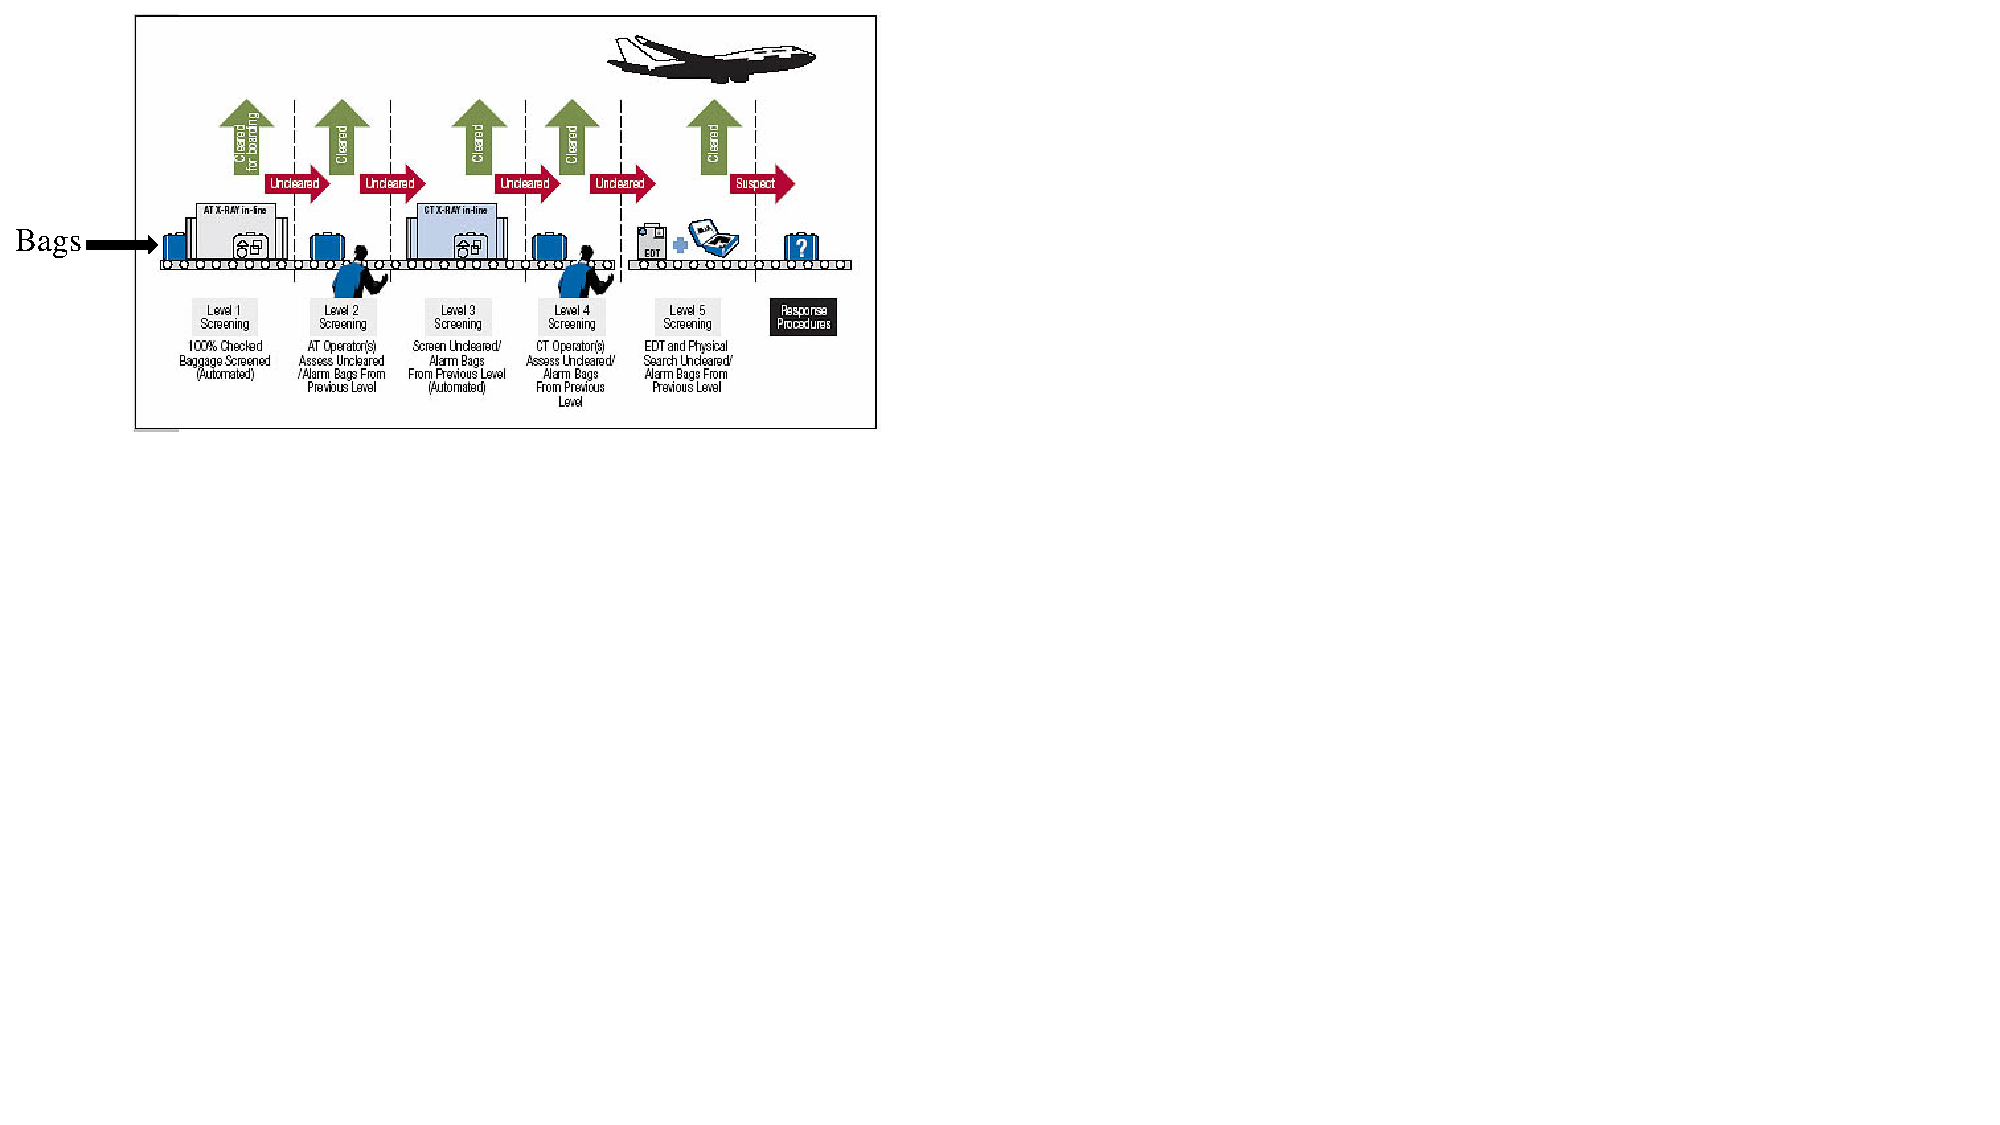
\includegraphics[width=0.4\textwidth]{../Figures/motiv.pdf}
  \caption{\footnotesize Sequential Sensor/Test Selection in Airport Security Systems. A number of different imaging and non-imaging tests are sequentially processed (see \cite{ML13_MultistageClassifier_TrapezSaligramaCastanon}). Costs can arise due to sensor availability and delay. Inexpensive tests are first conducted and based on their outcomes more expensive tests are conducted.}
  \label{motiv}
\vspace{-15pt}
\end{figure}
%Sensor-tests
%Many medical scenraios ranging from chronic diseases to real-time traumatic injury also involve a sequence of tests~\cite{baghdadian}. In the current triaging system the guidelines and standard of care for trauma patients are few and varied. The management of trauma is local and is often managed under institutional, rather than national guidelines~\cite{baghdadian,aastplenary}. In these applications the test 
%
The goal in these systems is to maximize overall accuracy for an available cost-budget. Generally, the components that can be optimized include sensor classifiers (to improve test accuracy), sensor ordering, and decision strategies for sequential \ses. Nevertheless, sensor classifiers and sensor ordering are typically part of the infrastructure and generally harder to control/modify in both security and medical systems. To this end we focus here  on the sequential \ses problem and use the terms sensor and test interchangeably. The need for systematically learning optimal decision strategies for balancing accuracy \& costs arises from the fact that these applications involve legacy systems where sensor/test selection strategies are local; often managed under institutional, rather than national guidelines~\cite{baghdadian}. %Consequently, systematic techniques for learning optimal decision strategies are required. 
While it is possible to learn such decision strategies given sufficient annotated training data, what makes these applications challenging is that it is often difficult to acquire in-situ ground truth labels. 

These observations motivate the problem of learning decision strategies for optimal \ses in situations where we do not have the benefit of ground-truth annotations, and what we refer to as the Unsupervised Sensor Selection (USS) problem. %We assume that the scenario is played over multiple rounds with an instance associated with each round. Each SBT outputs a prediction of the underlying state of the instance (anomaly, threat, disease or nominal etc.) and must be acquired sequentially complying with the cascade architecture in each round. The learner's goal is to figure out the hidden, stochastic state of the instance based on the sensor outputs. Since the learner knows that the sensors are ordered from least to most accurate he/she can use the most accurate sensor among his/her acquired sensors for prediction. Nevertheless, since the learner does not know the sensor accuracy he/she faces the dilemma of as to which sensor to use for predicting this state.
In \cref{sec:Setup} we pose our problem as a version of stochastic partial monitoring problem \cite{BaFoPaRaSze14} with \emph{atypical} reward structure, where tests are viewed as actions and sequential observations serve as side information. As is common, we pose the problem in terms of competitive optimality. We consider a competitor who can choose an optimal test with the benefit of hindsight. Our goal is to minimize cumulative regret based on learning the optimal test based on observations in multiple rounds of play. %Stochastic partial monitoring problem is itself a generalization of multi-armed bandit problems, the latter going back to \cite{Tho33}. The availability of predictions of parent sensors of a chosen sensor is viewed as side observation.  
Recall that in a stochastic partial monitoring problem a decision maker needs to choose the action with the lowest expected cost by repeatedly trying the actions and observing some feedback.
The decision maker lacks the knowledge of some key information, such as in our case, the misclassification
error rates of the classifiers, but had this information been available, the decision maker could calculate the
expected costs of all the actions (\ses{}s) and could choose the best action (test). The feedback received by the decision maker in a given round depends stochastically on the unknown information and the action chosen.
Bandit problems \cite{Tho33} are a special case of partial monitoring, where the key missing information is the expected
cost for each action, and the feedback is the noisy version of the expected cost of the action chosen.
In the USS problem the learner only observes the outputs of the classifiers, but not the label to be predicted over multiple rounds
in a stochastic, stationary environment. 


%To cast our problem as a partial monitoring problem, \todoc{Do we need this? Or leave this to the reader, just saying that casting our problem as a partial monitoring problem is trivial?} 
%the key unknown information can be the misclassification error rates of the classifiers, an action is identified with 
%the subset of sensors selected, the cost of an action is the sum of the misclassification cost of the classifiers
%that uses the selected sensor subset outputs and the cost of acquiring these sensor outputs,
%while the observed feedback is the vector of predicted labels by each of the classifiers that use 
%the first, the first and second, etc., up to all sensor outputs from the sensors that were selected.
%Note that unlike in a conventional bandit problem, we do not get \emph{direct} 
%feedback of how well our action performed (either noisy or noiseless)\footnote{This problem naturally arises in the surveillance and medical domains. We can perform a battery of tests on an individual in an airport but can never be sure whether or not he/she poses a threat.}.

%Were the probability of error known for each classifier that uses an initial segment of the tests, 
%a decision maker could optimally balance the cost of erroneous decisions and that of the \sess'.
%\todoc{This assumes a cost associated with each error; should this be noted?}
%In the learning version of the problem, the misclassification probabilities are \emph{a priori} unknown and a learner must learn the optimal balance based on some feedback available to him. 
%In the \emph{unsupervised} version considered here
%and which we call the unsupervised \emph{sequential \ses problem} (SAP),
%the learner only observes the outputs of the classifiers, but not the label to be predicted over multiple rounds
%in a stochastic, stationary environment. 

%This leads us to the following question: Can a learner still achieve the optimal balance in this case?  
In \cref{sec:Learnability} we first show (unsurprisingly) that no learner can achieve sublinear regret without further assumptions. To this end we propose the notions of weak and strong dominance, which correspond to constraints on joint probability distributions over the latent state and test-outcomes. Strong Dominance (SD) is a property arising in many engineered systems and says that whenever a test is accurate on an example, a later test in the sequence is almost surely accurate on that example. %(in other words a child SBT cannot make an error when the parent node is accurate). 
Weak Dominance (WD) is a relaxed notion that allows for errors in these predictions. We empirically demonstrate that WD holds by evaluating it on several real datasets. We also show that WD is fundamental in the sense that while there exist learners that achieve sublinear regret over WD instances, no new instances can be added to this class without losing this property.
%on this class (non-uniform) sublinear regret learner  without this condition there exist problem instances that result in linear regret. On the other hand whenever this condition is satisfied there exist algorithms that lead to sublinear regret. 

%In particular, we reduce the SAP problem to a stochastic multi-armed bandit with side observations, 
%a problem introduced by \citet{MaSh11}.
In \cref{sec:Equiv} under SD we show that USS is reducible to a version of multi-armed bandit problem (MAB) with side-observation, a problem that is known to be learnable with  sub-linear regret. In our reduction, we identify tests as bandit arms. % are identified by the nodes of the cascade. \todoc{Should we introduce cascade formally then above?}
The payoff of an arm is given by marginal losses relative to the root test, and the side observation structure is defined by the feedback graph induced by the directed graph. We then formally show that there is a one-to-one mapping between algorithms for USS and algorithms for MAB with side-observation. In particular, under SD, the regret bounds for MAB with side-observation then imply corresponding regret bounds for USS. \todoc{This said WD, but that's not true, right?}

%\noindent
\subsection{Related Work}
%
%Supervised, batch learning, the problem is well studied.
%
In contrast to our USS setup there exists a wide body of literature dealing with \ses (see \cite{AISTATS13_SupervisedSequentialLearning_TrapezSaligram}). Like us they also deal with cascade models with costs for features/tests but their method is based on training decision strategies with fully supervised data. There are also several methods that work in an online bandit setting and train prediction models with feature costs \cite{SBCA14:BanditsPaid} but again they require true labels as reward-feedback. A somewhat more general version of \cite{SBCA14:BanditsPaid} is developed in  \cite{ZBGGySz13:CostlyFeatures} where in addition the learner can choose to acquire true labels for a cost.

%
%However, unlike us these works focus on prediction-time cost/accuracy tradeoffs, which assumes a fully labeled training set for test-time use. %In particular they assume that a fully labeled training dataset is provided for test-time use. 

Our paper bears some similarity with the concept of active classification, which deals with learning stopping policies \cite{poczos2009,ActiveClass-AIJ-s} among a given sequence of tests. Like us these works also consider costs for utilizing tests and the goal is to learn when to stop to make decisions. Nevertheless, unlike our setup the loss associated with the decision is observed in their context. %when a decision is made. 
%
%
%decide when to quit a cascade that leads to better decisions to maximize throughput against error rates. Again full feedback with accuracy of classification is assumed. Our problem is somewhat related to active classification. Nevertheless, while methods as in \cite{ActiveClass-AIJ-s} seek a classifier that decides what tests to take given the results of previous tests to minimize total cost, they also exclusively deal with batch-supervised learning in this context. The same setting is also studied under hard budget constraints in \cite{LCunderBudget-ECML05}.% and its applications in imaging and computer vision systems are explored in  \cite{ADORE-99,isukapalli01efficient-ICJAI}).
% \todoc{I suspect they assume more than this:
% 	In our previous paper we had a sentence that said that
% 	``their model requires knowing a model of the actions in 
% 	advance'' (this would mean knowing the joint probabilities, I think).}
%  \todoc{Actually, much work exists, need to google this}\todom{Added a line about each reference, not sure if we need to include more similar references}
%
%
%The prediction-time learning \cite{SBCA14:BanditsPaid}, the decision maker can opt to pay for additional observations of the costs associated with other arms. Unlike ours this setting is not unsupervised. In
%\cite{ZBGGySz13:CostlyFeatures}, online learning with costly features and labels is studied.
%In each round, learner has to decide which features to observe, where each feature costs some money. The learner can also decide not to observe the label, but the learner always has the option
%to observe the label. Again this setting is not unsupervised.

%Partial monitoring:
Our paper is related to the framework of finite partial monitoring problems \cite{BaFoPaRaSze14}, which deals with how to infer unknown key information and where tests/actions reveal different types of information about the unknown information. In this context 
%applies to the so-called finite problems (unknown ``key information'') is an element of the probability simplex.
\cite{AgTeAn89:pmon} consider special cases where payoff/rewards for a subset of actions are observed. This is further studied as a side-observation problem in \cite{MaSh11} and as graph-structured feedback \cite{COLT15_OnlineLearningWithFeedback_AlonBianchiDekel, NIPS13_FromBanditsToExperts_AlonBianchiGentile,WGySz:NIPS15}. Our work is distinct from these setups because we are unable to observe rewards for our chosen actions or any other actions.
\vspace{-10pt}
%corresponding to chosen actions (whether the chosen action or in terms of side observations 
%\todom{Need to add Yifan's paper, there seems to be few more based on this in ICML'16, AISTATS'16 and NIPS'16}

%The paper is organized as follows: in Section \ref{sec:background} we give a brief background on online learning problems and discuss information structure in these setups. In Section \ref{sec:Setup} we introduce SAP as a general online learning problem where feedback reveals no information on loss/reward of actions. In Sectjon \ref{sec:Learnability} we identify conditions under which optimal action can be learned in SAP. In Section \ref{sec:Equiv} we establish that SAP is regret equivalent to a stochastic multi-armed bandits with side-observations when it satisfies strong dominance property. When this property holds, Section \ref{sec:Algo} gives an algorithm to solve SAP efficiently. We conclude in Section \ref{sec:Conclu} with a discussion on further extensions.  